\documentclass[a4paper,12pt]{report}

\usepackage[utf8x]{inputenc}
\usepackage[T2A]{fontenc}
\usepackage[english, russian]{babel}
\usepackage{verbatim}
\usepackage{pdfpages}

% Опционно, требует  apt-get install scalable-cyrfonts.*
% и удаления одной строчки в cyrtimes.sty
% Сточку не удалять!
% \usepackage{cyrtimes}

% Картнки и tikz
\usepackage{graphicx}
\usepackage{tikz}
\usetikzlibrary{snakes,arrows,shapes}


% Увы, поля придётся уменьшить из-за листингов.
\topmargin -1cm
\oddsidemargin -0.5cm
\evensidemargin -0.5cm
\textwidth 17cm
\textheight 24cm

\sloppy



% Оглавление в PDF
\usepackage[
bookmarks=true,
colorlinks=true, linkcolor=black, anchorcolor=black, citecolor=black, menucolor=black,filecolor=black, urlcolor=black,
unicode=true
]{hyperref}

% Для исходного кода в тексте
% \newcommand{\Code}[1]{\texttt{#1}}

% Некоторая русификация.
% \usepackage{misccorr} % Oh shi^W^W, оно не работает с report.
\usepackage{indentfirst}
\renewcommand{\labelitemi}{\normalfont\bfseries{--}}

% На дворе XXI век, но пакет listings всё ещё не пашет с русскими комментариями!

% Пакет listings для простой вставки исходников
% \usepackage{listings}
% Параметры оформления
% \lstset{
% showspaces=false,
% showtabs=false,
% frame=single,
% tabsize=4,
% basicstyle=\ttfamily,
% identifierstyle=\ttfamily,
% commentstyle=\itshape,
% stringstyle=\ttfamily,
% keywordstyle=\ttfamily,
% breaklines=true
% }
% Русский в комментариях.
% \lstset{escapebegin=\begin{cyr},escapeend=\end{cyr}}



% А это взято из файла, сгенерённого doxygen
\usepackage{calc}
\usepackage{array}
\newenvironment{Code}
{\footnotesize}
{\normalsize}
\newcommand{\doxyref}[3]{\textbf{#1} (\textnormal{#2}\,\pageref{#3})}
\newenvironment{DocInclude}
{\footnotesize}
{\normalsize}
\newenvironment{VerbInclude}
{\footnotesize}
{\normalsize}
\newenvironment{Image}
{\begin{figure}[H]}
{\end{figure}}
\newenvironment{ImageNoCaption}{}{}
\newenvironment{CompactList}
{\begin{list}{}{
  \setlength{\leftmargin}{0.5cm}
  \setlength{\itemsep}{0pt}
  \setlength{\parsep}{0pt}
  \setlength{\topsep}{0pt}
  \renewcommand{\makelabel}{\hfill}}}
{\end{list}}
\newenvironment{CompactItemize}
{
  \begin{itemize}
  \setlength{\itemsep}{-3pt}
  \setlength{\parsep}{0pt}
  \setlength{\topsep}{0pt}
  \setlength{\partopsep}{0pt}
}
{\end{itemize}}
\newcommand{\PBS}[1]{\let\temp=\\#1\let\\=\temp}
\newlength{\tmplength}
\newenvironment{TabularC}[1]
{
\setlength{\tmplength}
     {\linewidth/(#1)-\tabcolsep*2-\arrayrulewidth*(#1+1)/(#1)}
      \par\begin{tabular*}{\linewidth}
             {*{#1}{|>{\PBS\raggedright\hspace{0pt}}p{\the\tmplength}}|}
}
{\end{tabular*}\par}
\newcommand{\entrylabel}[1]{
   {\parbox[b]{\labelwidth-4pt}{\makebox[0pt][l]{\textbf{#1}}\vspace{1.5\baselineskip}}}}
\newenvironment{Desc}
{\begin{list}{}
  {
    \settowidth{\labelwidth}{40pt}
    \setlength{\leftmargin}{\labelwidth}
    \setlength{\parsep}{0pt}
    \setlength{\itemsep}{-4pt}
    \renewcommand{\makelabel}{\entrylabel}
  }
}
{\end{list}}
\newenvironment{Indent}
  {\begin{list}{}{\setlength{\leftmargin}{0.5cm}}
      \item[]\ignorespaces}
  {\unskip\end{list}}


\title{Рассчётно-пояснительная записка к курсовой работе
       "Разработка SMTP клиента"}
\author{Килочек Ю.И.}

\begin{document}

\maketitle

\tableofcontents

\cleardoublepage
\phantomsection
\addcontentsline{toc}{chapter}{Введение}
\chapter*{Введение}

Задание:
\begin{itemize}
\item Создание SMTP-клиента (как части MTA), обеспечивающего удаленную доставку
      и поддерживающего очереди сообщений.
\item Отправитель должен поддерживать набор команд, достаточный для отправки
      почты как минимум одной крупной почтовой публичной службе с
      веб-интерфейсом (по выбору студента).
\item Все варианты предполагают обработку нескольких исходящих соединений в
      одном потоке выполнения (т.е., одном процесс или одном потоке).
\item На один удалённый MX надо создавать не более одного сокета (допустимый
      вариант — на один удалённый IP не более одного сокета).
\item Следует использовать отдельную очередь собщений для каждого MX.
\item Вариант 29: Используется вызов poll и единственный рабочий поток (или
      процесс). Журналирование в отдельном потоке. Пытаться отправлять все
      сообщения для одного MX за одну сессию.
\end{itemize}

Цель работы~-- Создание SMTP-клиента (как части MTA), обеспечивающего удаленную
доставку и поддерживающего очереди сообщений.

Для достижения поставленной цели необходимо решить следующие задачи: 
\begin{itemize}
\item Изучение протокола SMTP по имеющейся спецификации.
\item Реализация SMTP клиента на языке С99.
\item Автоматизированное системное тестирования разработанного ПО. 
\item Тестирования утечек памяти.
\item Создание сценариев сборки ПО.
\end{itemize}

\chapter{Аналитический раздел}

\section{Достоинства и недостатки указанных в задании подходов к решению задачи}

Достоинства:
\begin{itemize}
\item Мультиплексирование снимает нагрузку с процессора (как при активном
      ожидании) и более легковесно чем создание отдельных процессов/потоков.
\item \texttt{poll}~-- часть стандарта \texttt{POSIX}.
\item Отсутствие веременных затрат на разрыв и повторную установку соединения
      в случае, когда несколько писем необходимо доставить на один и тот же
      почтовый сервер.
\end{itemize}

Недостатки:
\begin{itemize}
\item \texttt{poll} имеет линейную сложность, на Linux существует более
      совершенный механизм~-- \texttt{epoll}.
\item Вынос журналирования в отдельный поток при использовании
      мультиплексирования не дает прироста производительности.
\item Необходимость синхронизации потоков.
\item Более сложный алгоритм работы.
\end{itemize}

\section{Сущности предметной области}

В результате проведённого исследования были выделены следующие сущности
предметной области (рисунок ~\ref{fig:entities}).

\begin{figure}
\centering
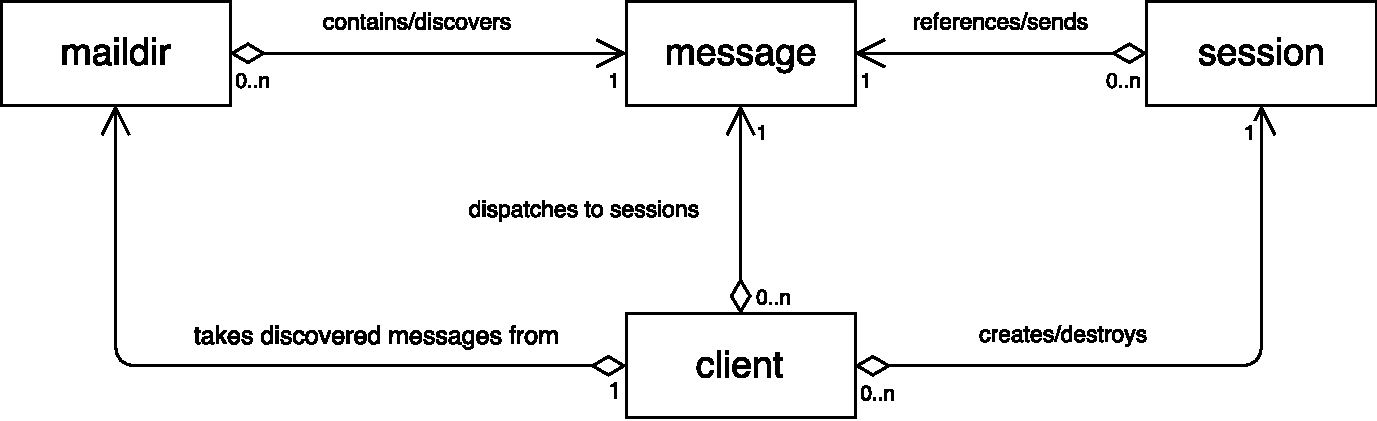
\includegraphics[width=\textwidth]{report/entities.pdf}
\caption{Основные сущности предметной области}
\label{fig:entities}
\end{figure}

\chapter{Конструкторский раздел}

\section{Конечный автомат состояний сессии}

Конечный автомат состояний клиента представлен на рисунке ~\ref{fig:fsm}. Для
того чтобы улучшить его читаемость были опущены переходы из всех состояний в
состояние ошибки.

\begin{figure}
\centering
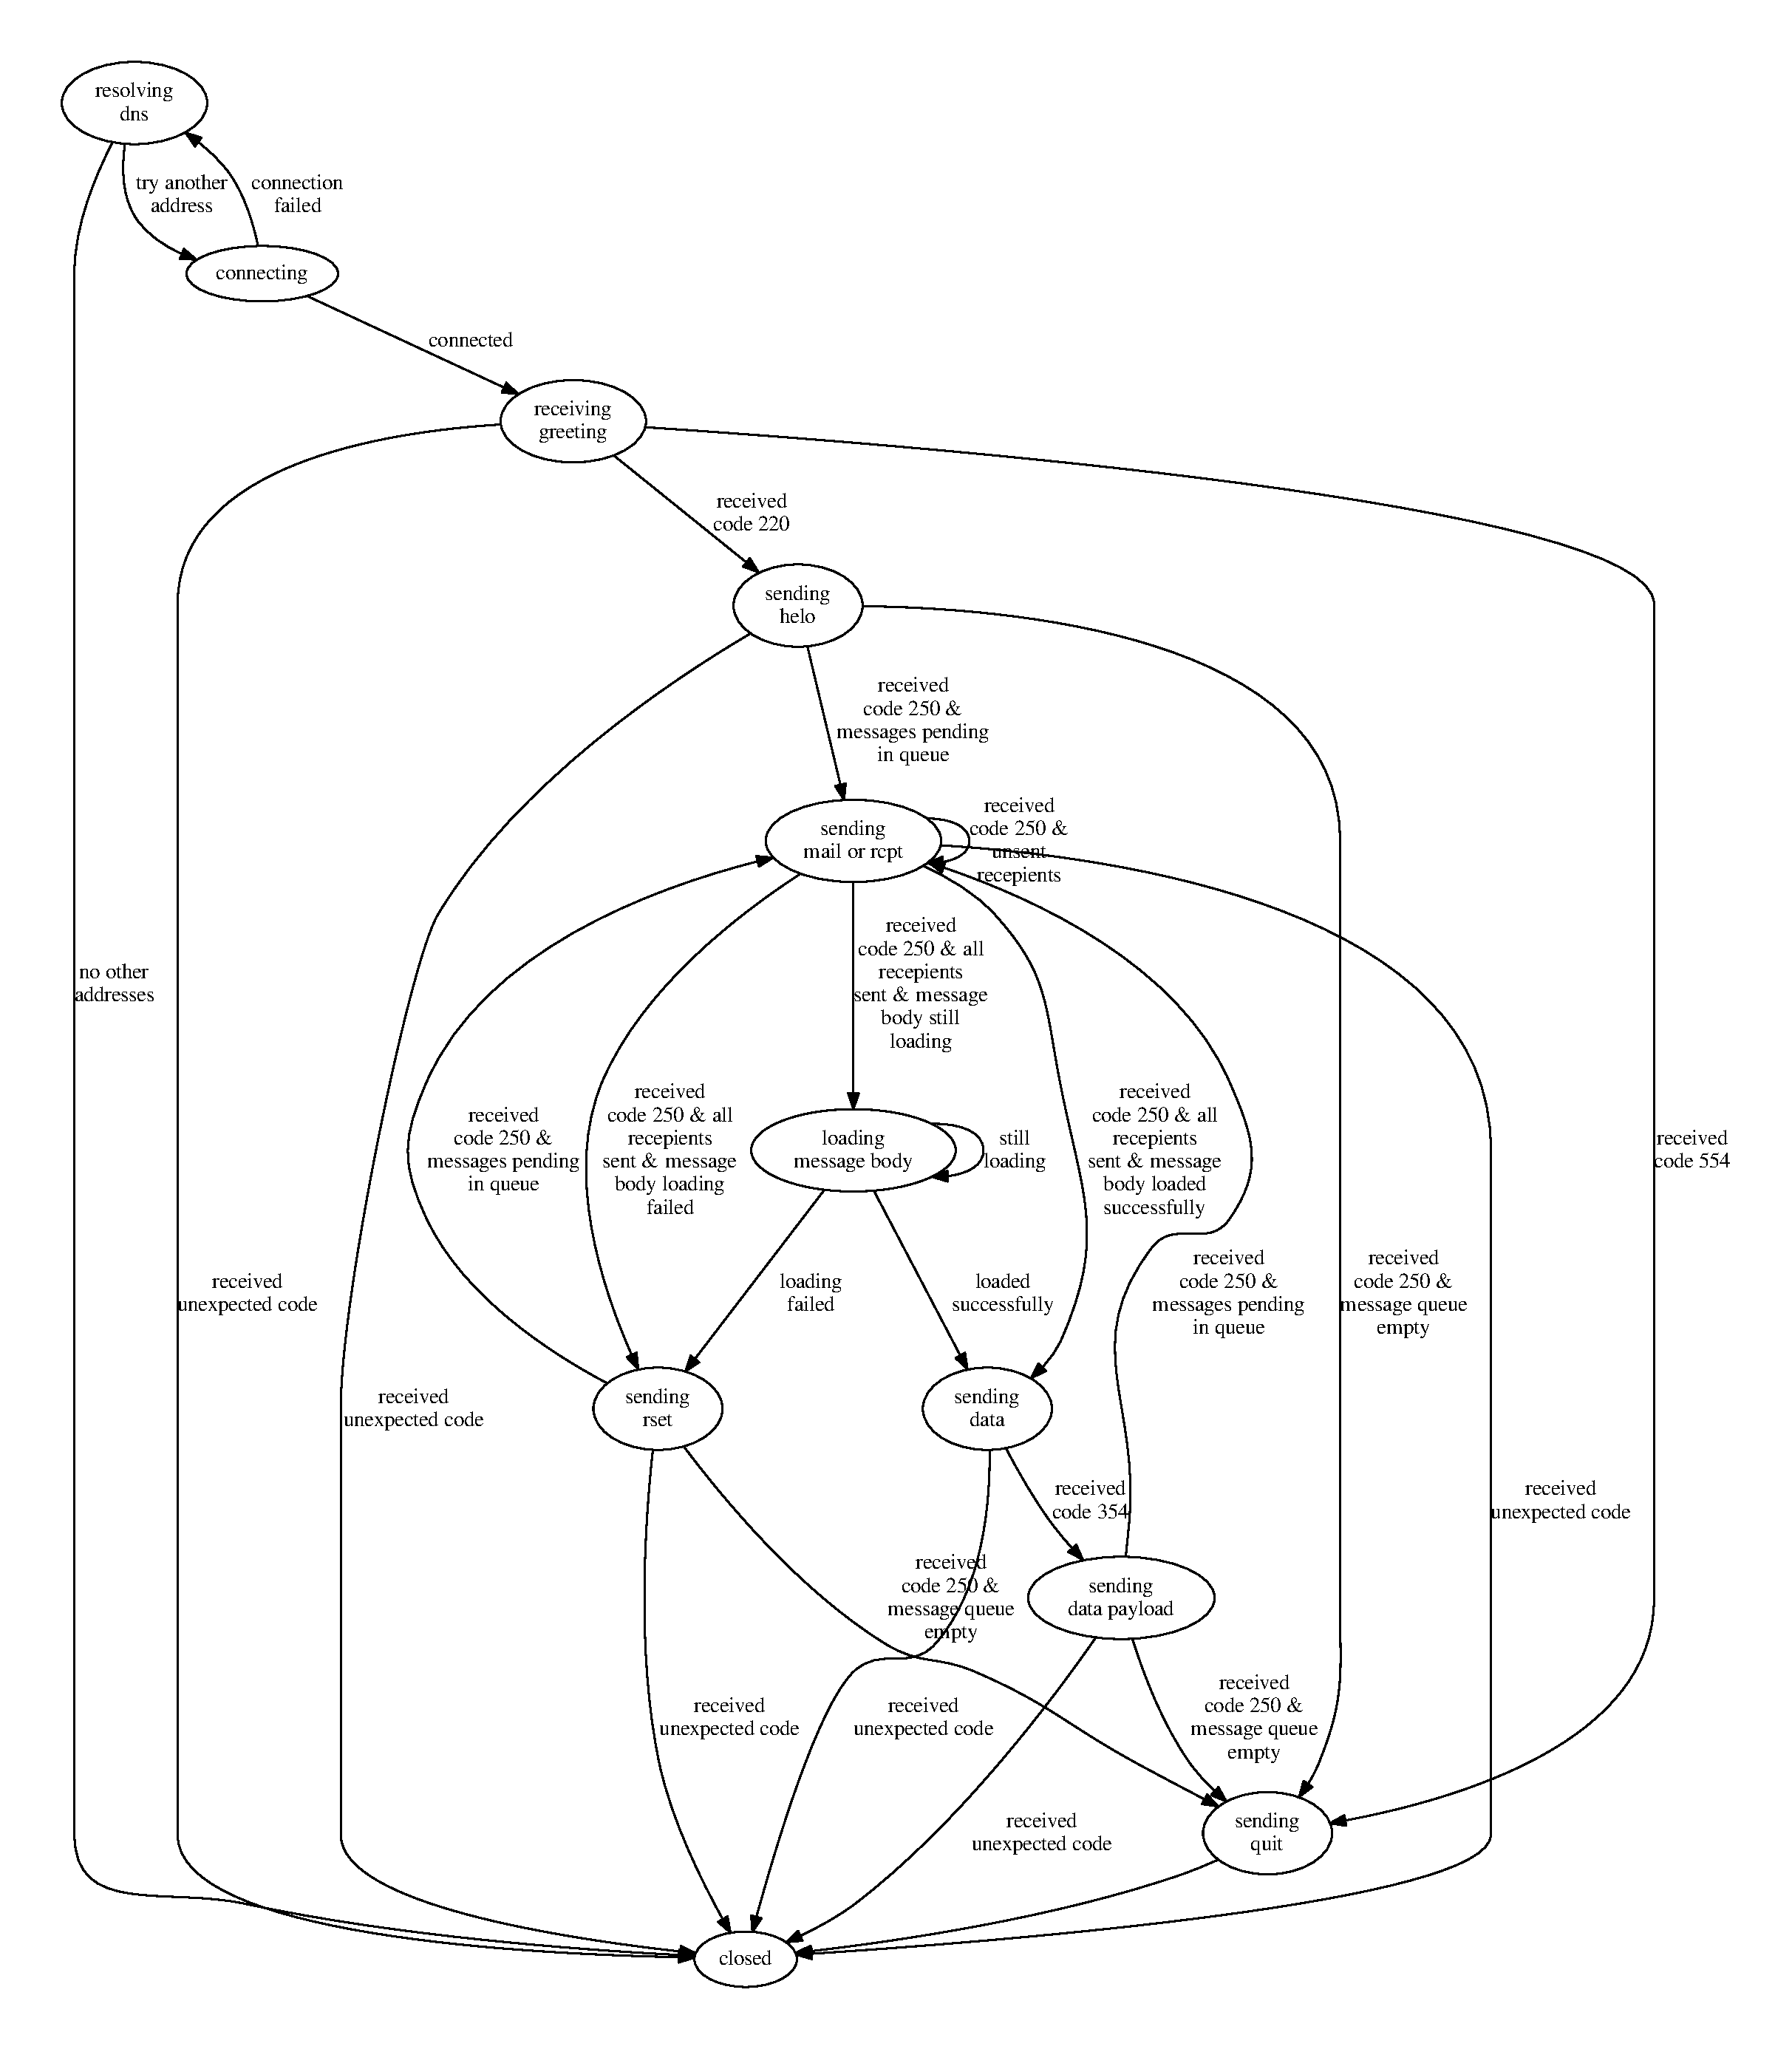
\includegraphics[width=\textwidth]{.tmp/report/fsm.pdf}
\caption{Конечный автомат состояний клиента}
\label{fig:fsm}
\end{figure}

\section{Взаимодействие подсистем}

На диаграмме последовательности действий (рисунок ~\ref{fig:activity})
изображён стандартный процесс обнаружения нового сообщения в maildir и его
дальнейшей отправки по адресу назначения:

\begin{figure}
\centering
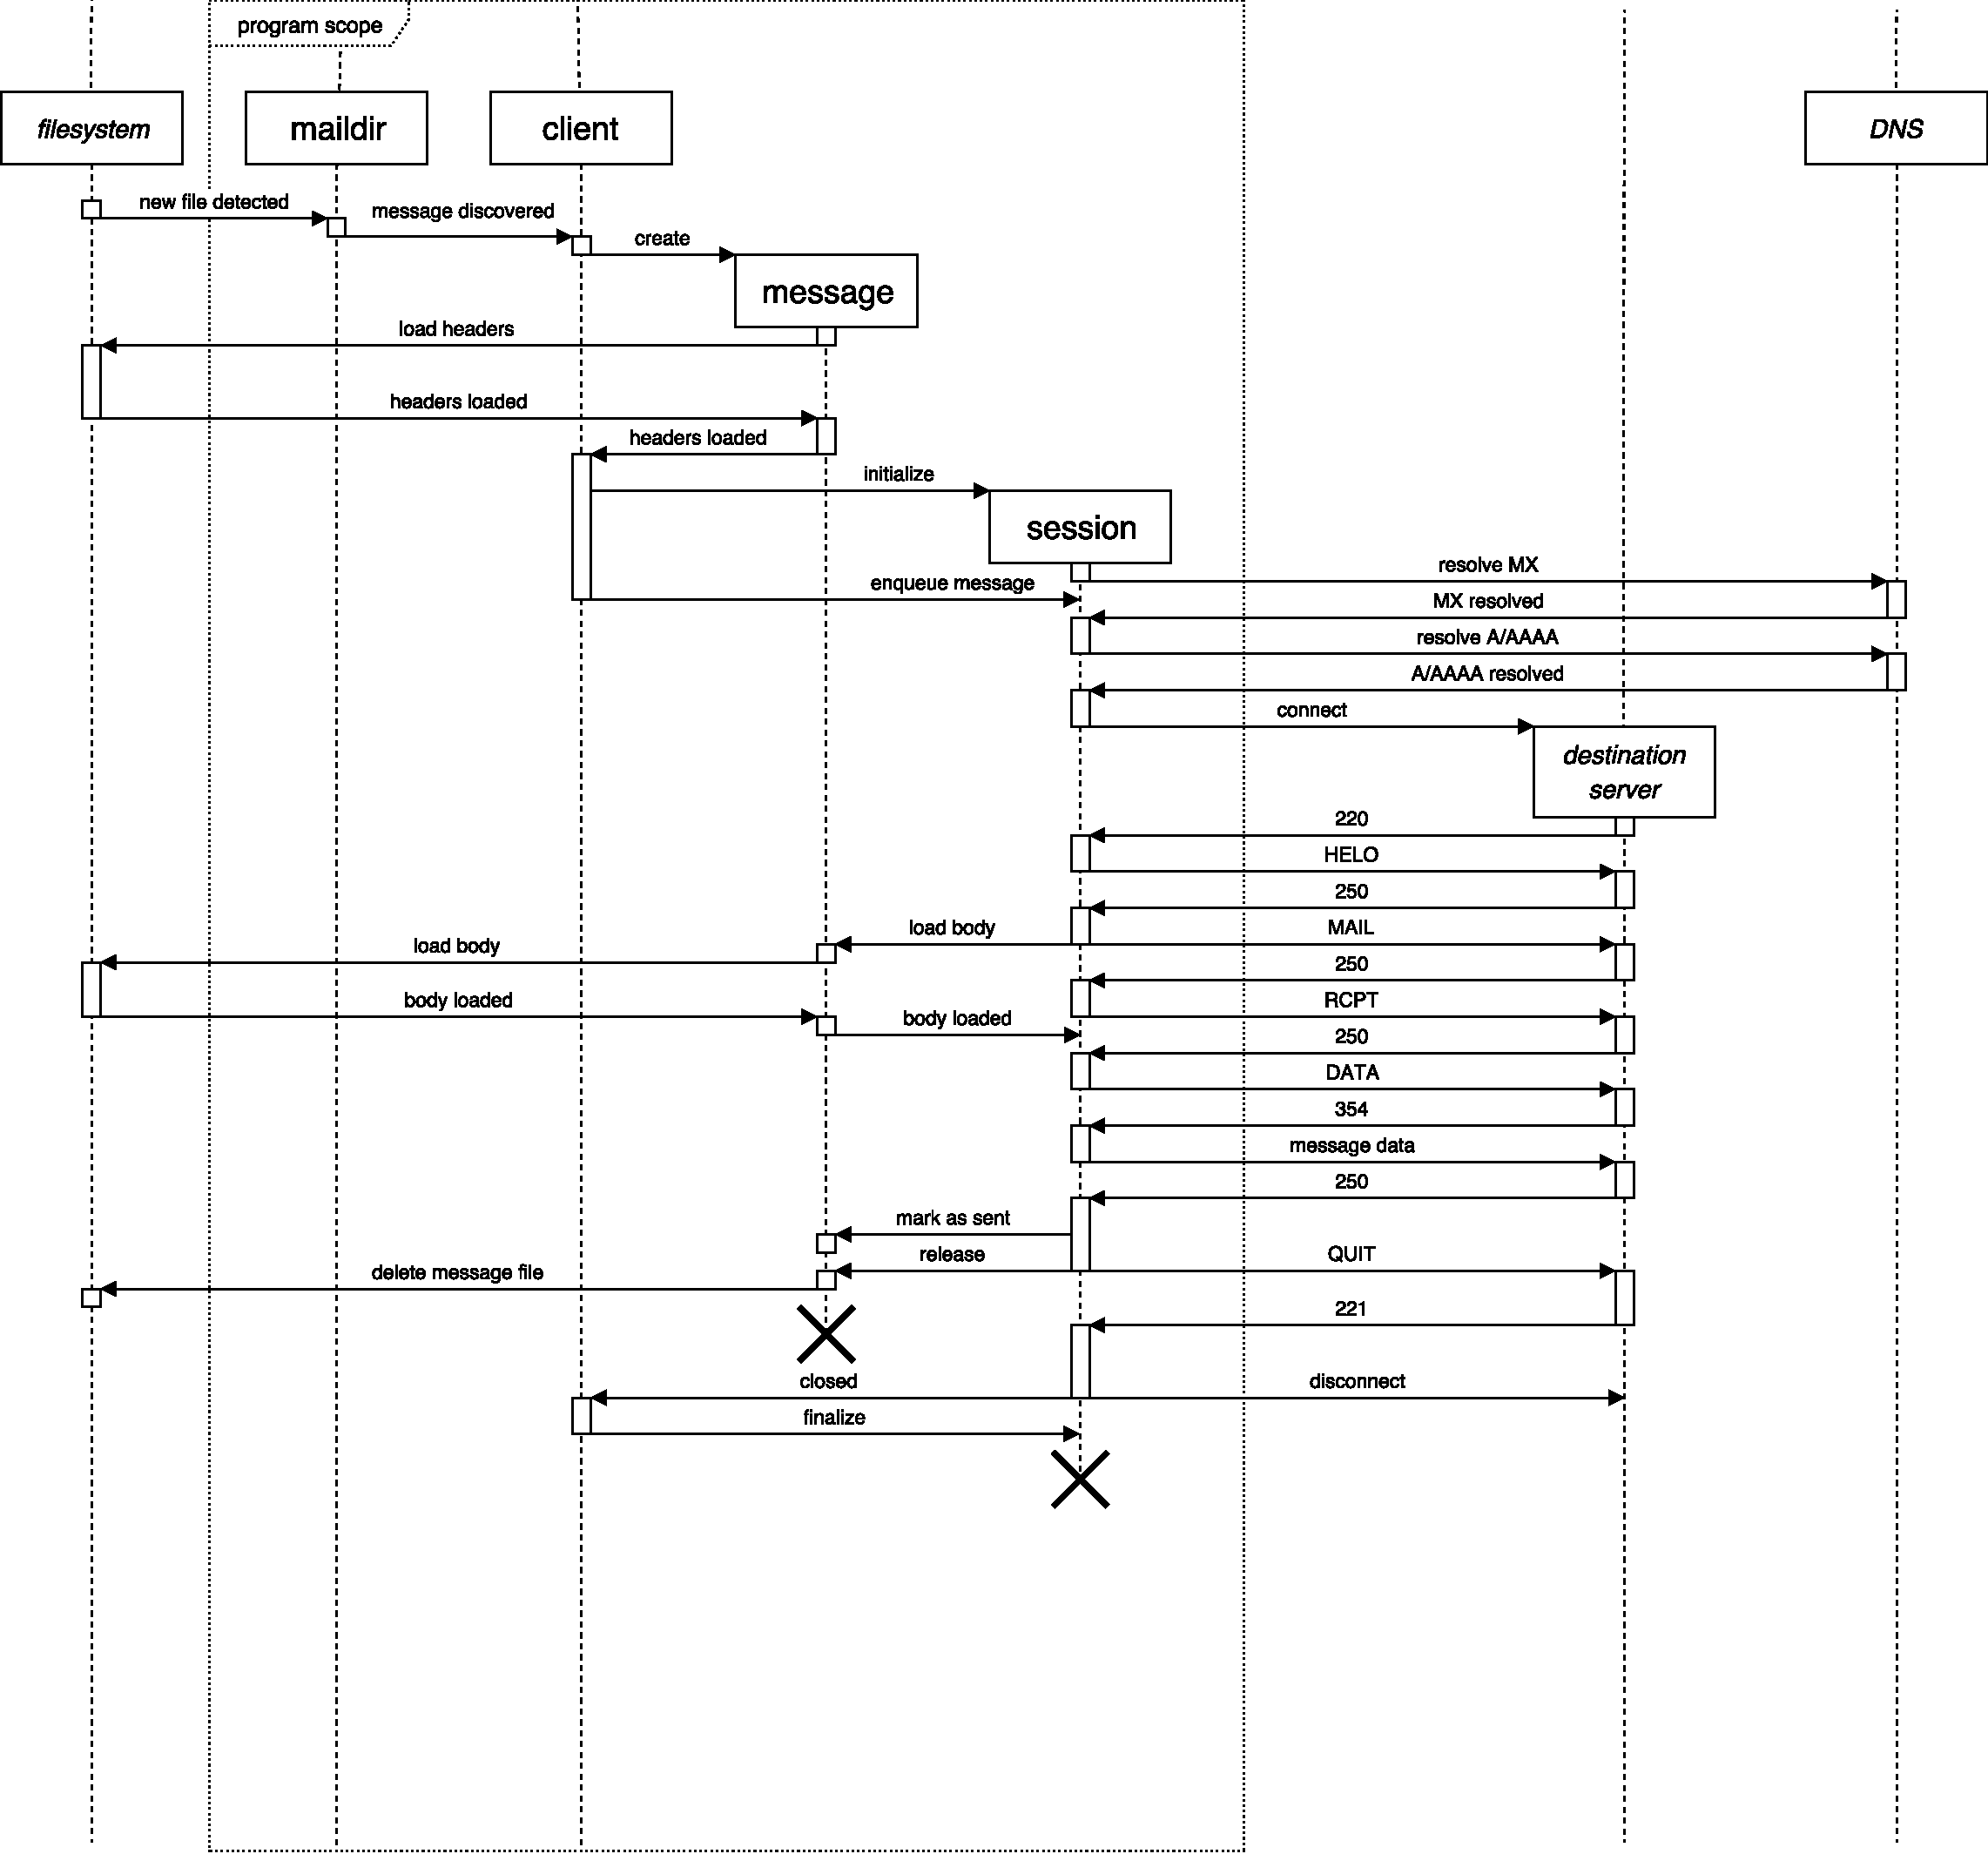
\includegraphics[width=\textwidth]{report/activity.pdf}
\caption{Диаграмма последовательности действий при нормальной отправке
         сообщения}
\label{fig:activity}
\end{figure}

\section{Синхронизация потоков}

Так как журналирование вынесено в отдельный поток выполнения, необходима
синхронизация между ним и основным потоком для безопасного доступа обоих к
очереди сообщений журнала. Это достигается с помощью стандартного механизма
\texttt{mutex}/\texttt{condition variable}.

\chapter{Технологический раздел}

\section{Cборка}

Зависимости:
\begin{itemize}
\item \texttt{c-ares}
\item \texttt{python2}
\item \texttt{python3} + \texttt{pipenv} (после установки выполнить
      \texttt{pipenv install})
\item \texttt{valgrind}
\item \texttt{cflow}
\item \texttt{graphviz}
\item \texttt{texlive}
\end{itemize}

Сборка исполняемого файла клиента (рисунок ~\ref{fig:dependencies})
производится с помощью GNU make, \texttt{Makefile} размещен в корневой
директории и содержит цели:
\begin{itemize}
\item \texttt{client}~-- Сборка исполняемого файла клиента.
\item \texttt{report.pdf}~-- Сборка этого отчета.
\item \texttt{test\_system}~-- Системное тестирование под \texttt{valgrind}ом.
\item \texttt{all}~-- Выполение всех пунков выше.
\item \texttt{clean}~-- Удаление всех сгенерированных файлов.
\end{itemize}

\begin{figure}
\centering
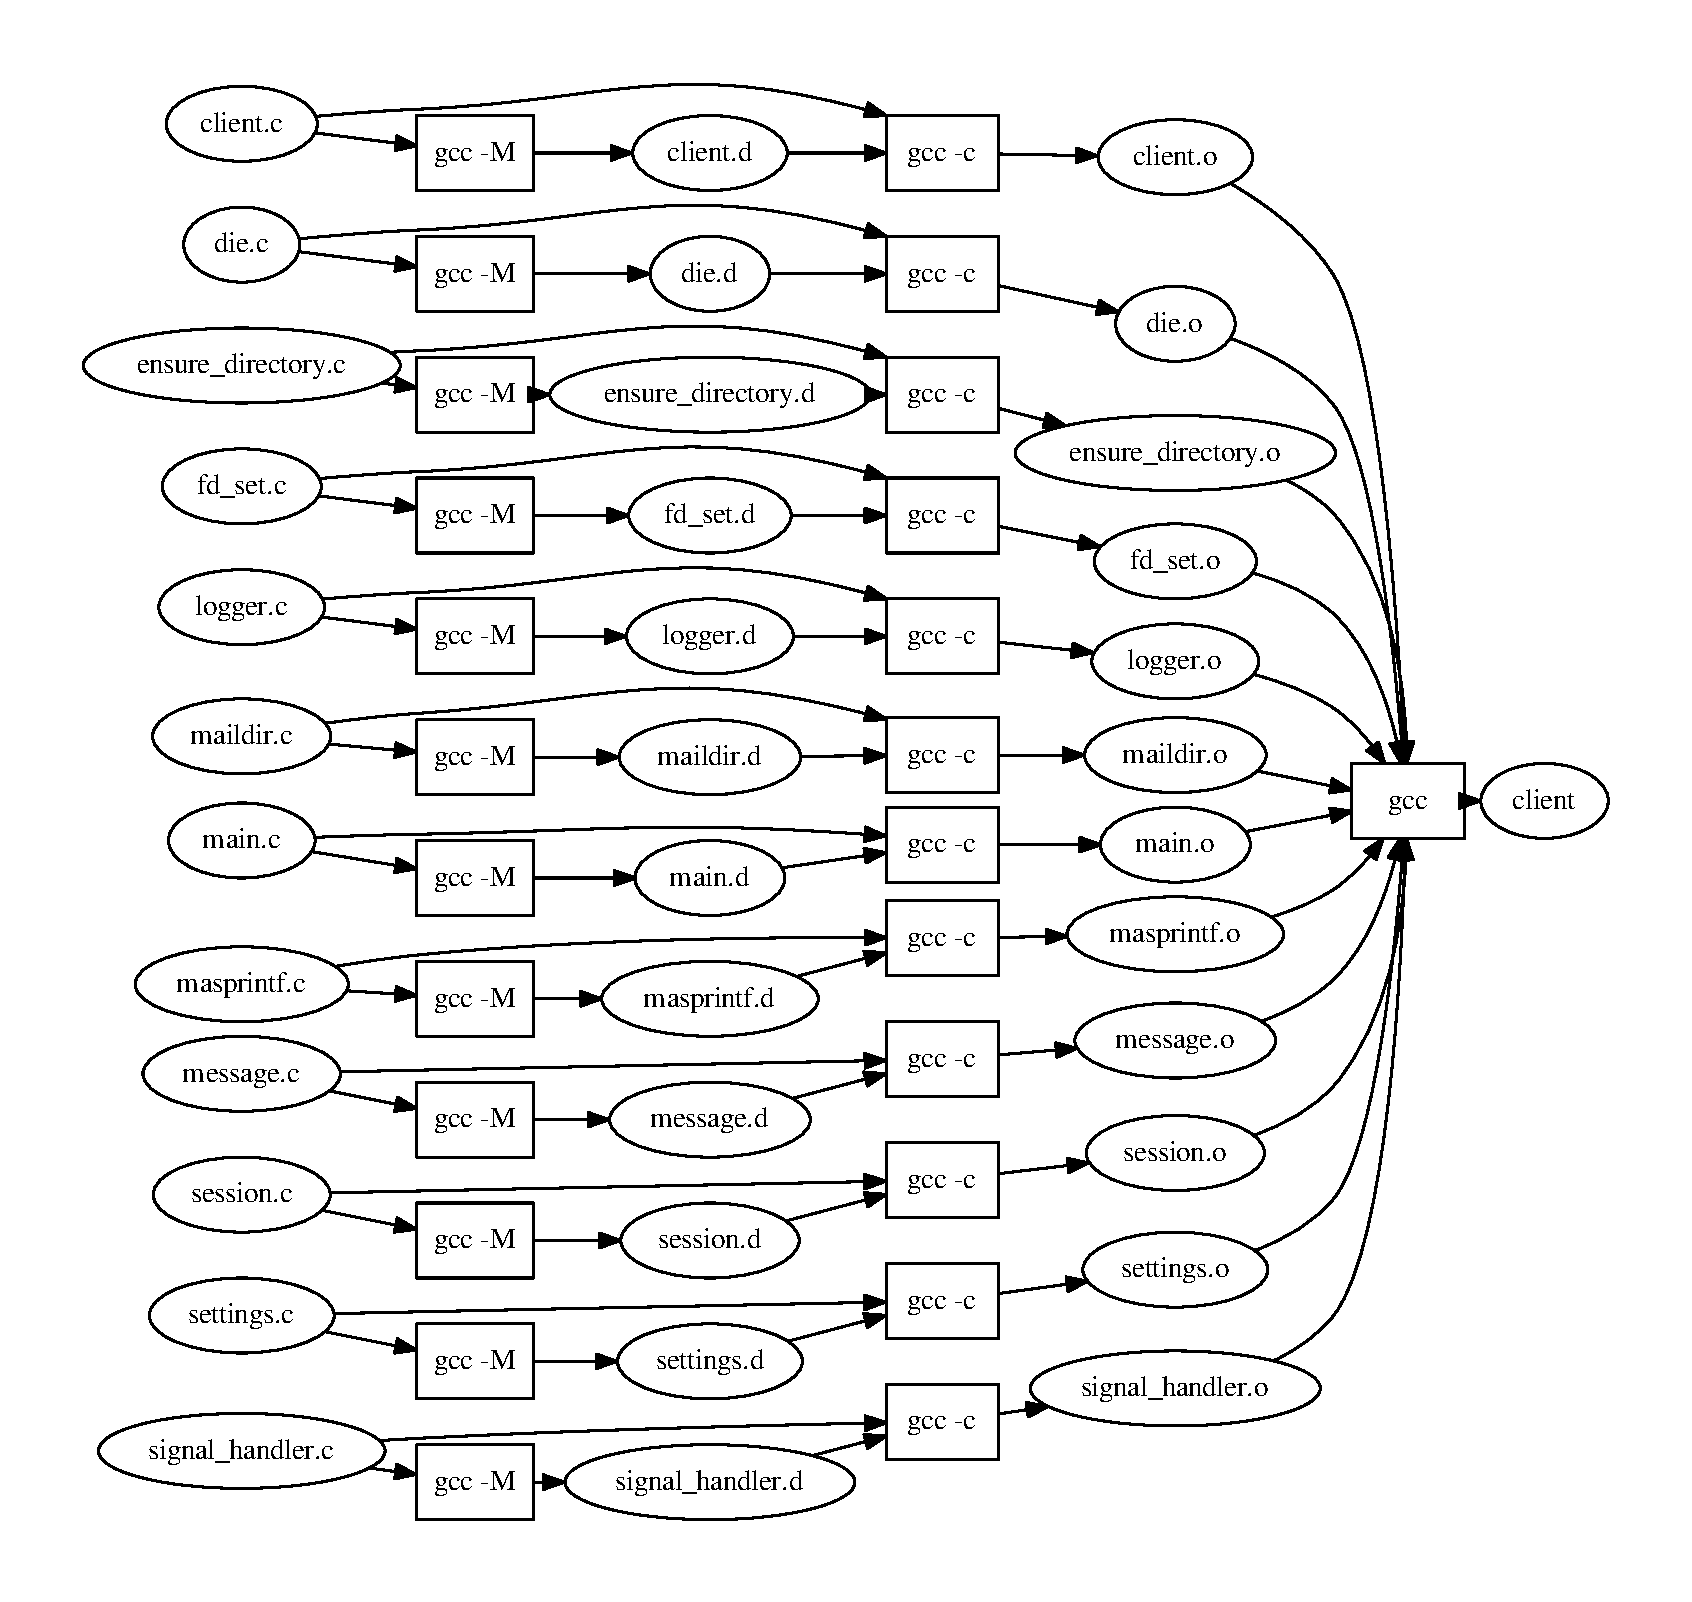
\includegraphics[width=\textwidth]{.tmp/report/dependencies.pdf}
\caption{Схема сборки исполняемого файла клиента}
\label{fig:dependencies}
\end{figure}

Схема сборки исполняемого файла клиента (рисунок~\ref{fig:dependencies})
сгенерирована автоматически из \texttt{Makefile}а утилитами
\texttt{report/tools/makesimple} и \texttt{report/tools/makefile2dot} и
\texttt{dot}.

Граф вызовов функций (рисунок~\ref{fig:flow}) сгенерирован автоматически
утилитами \texttt{cflow}, \texttt{report/tools/cflow2dot} и \texttt{dot}.

Работоспособность проверена на ОС \texttt{Arch Linux 4.14.12-1}.

\section{Граф вызовов функций}

Граф вызовов функций приведен на рисунке~\ref{fig:flow} (некоторые маловажные
вызовы опущены).
\begin{figure}
\centering
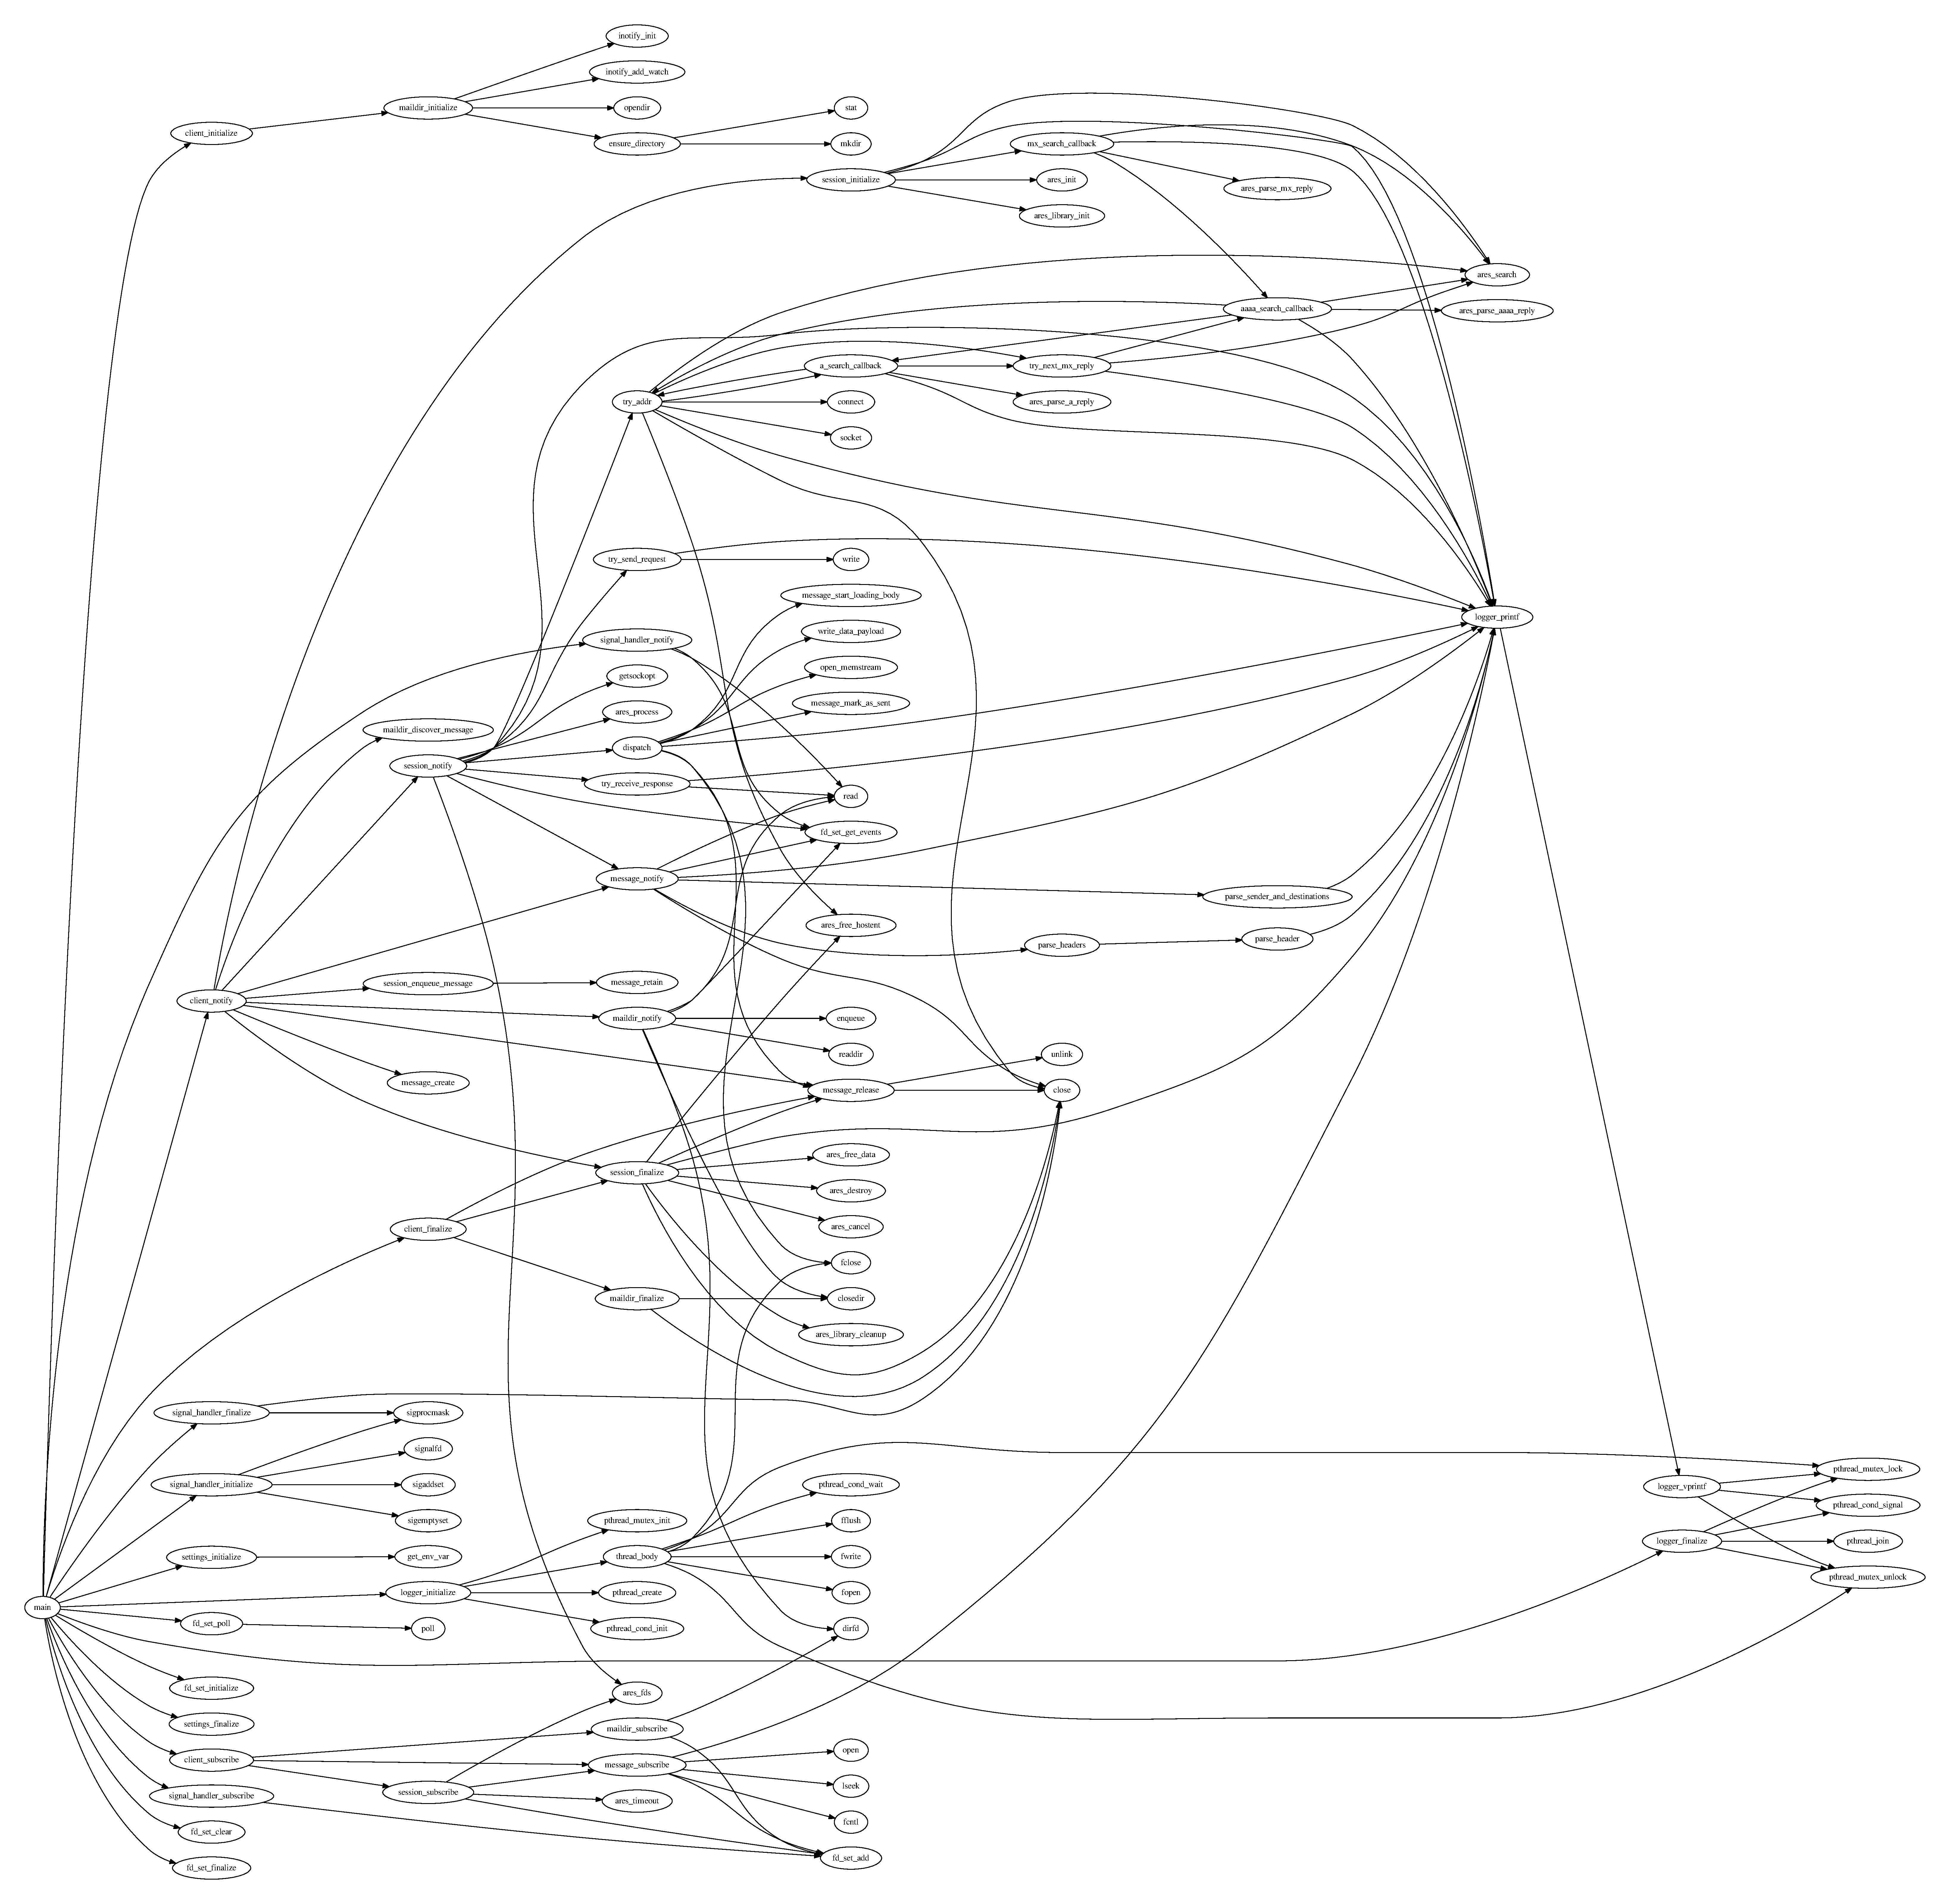
\includegraphics[width=\textwidth]{.tmp/report/flow.pdf}
\caption{Граф вызовов функций}
\label{fig:flow}
\end{figure}

\section{Настройки}

Конфигурация клиента осуществляется через переменные окружения:
\begin{itemize}
\item \texttt{SMTP\_CLIENT\_LOG}~-- Путь к файлу журнала (по умолчанию~--
      \texttt{/dev/stderr}).
\item \texttt{SMTP\_MAILDIR}~-- Путь к maildir каталогу (по умолчанию~--
      \texttt{maildir}).
\item \texttt{SMTP\_HOST}~-- DNS имя которым представляется клиент в SMTP
      команде \texttt{HELO} (по умолчанию~-- \texttt{localhost}).
\end{itemize}

\section{Тестирование}

Для проведения системного тестирования былa написана вспомгательная на языке
Python. Тест заключается в запуске клиента под \texttt{valgrind} для отправки
сообщения на сервер открытого почтовый сервиса \texttt{guerrilamail},
извлечении полученного им сообщения через HTTP API и сравнение его с
отправленным. Если сообщение получено успешно, совпадает с отправленным и при
работе клиента \texttt{valgrind} не обнаружил ошибок, то тест считается
пройденным.

Выполнение теста выглядит следующим образом:
\begingroup
\fontsize{10pt}{12pt}
\selectfont
\verbatiminput{.tmp/report/test_system.log}
\endgroup

\cleardoublepage
\phantomsection
\addcontentsline{toc}{chapter}{Выводы}
\chapter*{Выводы}

В результате выполнения курсового проекта достугнута поставленная цель~--
разработано приложение smtp-клиента, обеспечивающего удаленную доставку и
поддерживающего очереди сообщений.

В процессе достижения поставленной цели были решены следующие задачи: 
\begin{itemize}
\item Изучение протокола SMTP по имеющейся спецификации.
\item Реализация SMTP клиента на языке С99.
\item Автоматизированное системное тестирования разработанного ПО. 
\item Тестирования утечек памяти.
\item Создание сценариев сборки ПО.
\end{itemize}

\cleardoublepage
\phantomsection
\addcontentsline{toc}{chapter}{Приложение 1. Стрктуры данных и функции
    программы. (Сгенерировано Doxygen)}
\chapter*{Приложение 1. Стрктуры данных и функции программы. (Сгенерировано
    Doxygen)}

\includepdf[pages={3-11,13-27,29-54}]{.tmp/report/doxy/latex/refman.pdf}

\end{document}
